\section{Evaluation of real-time interactions between the user and the agent}
\label{sec:eval}

We present in this section an evaluation of real-time interactions between users and an embodied conversational agent in the context of a survival scenario.

\subsection{Motivation}

%In this section we present the evaluation of real-time interactions between an agent controlled by our turn-taking model and a user. We want to measure the effect of the variability of turn-taking strategies of our agent on the user experience of the interaction, especially regarding their comfort level interacting with the agent, or the credibility of the latter. We also want to assess the capability of our model to coordinate its turns with the user by evaluating the user's judgement on the ability of the agent to take into account the behavior of its partner. 
In this evaluation we had three research questions.  \begin{enumerate}
	\item Is an agent controlled by our turn-taking model able to coordinate smoothly its speaking turns with the user?
	\item Is an agent able to correctly signal its intentions (either taking, yielding keeping or grabbing the turn) to the user?
	\item Is an agent varying its turn-taking behavior according to our model improve judgements about the agent's credibility, user's satisfaction and easiness to interact with the agent?
\end{enumerate}

% of the interaction, especially regarding their comfort level interacting with the agent, or the credibility of the latter. 
%We also wanted to assess how users judged the ability of the agent to take into account the behavior of its partner.
To that purpose we chose to inspire from existing evaluations.
\cite{skantze_towards_2010} and \cite{de_vault_toward_2015} elaborated two experiments aiming at evaluating agent's turn-taking in the context of negociation scenarios. In these two experiments, the agents were at least partially controlled by a WoZ. In \cite{skantze_towards_2010} only the user's utterances were transcribed by the WoZ, the remaining being managed by the system. User's end of turns were identified using a simple voice activity detector and the system systematically responded to the user after detecting the end of the user's turn. In \cite{de_vault_toward_2015}, the whole process, from interpretation to generation, was managed by the Woz, including turn-taking behavior that was allowed to freely vary. These two experiments have the advantage to answer similar research questions as ours regarding turn-taking. First, the ability of the agent to coordinate with the user is evaluated by comparisons of the agent's response time and overlap duration with human interactions. Second, the agent's credibility, the user's satisfaction and easiness to interact with the agent are evaluated through questionnaire. Moreover, while the ability of the agent to correctly signals its intentions towards turn-taking are not directly treated, some behaviors of the user are assessed in these evaluations such as the user response time after the end of the agent's turn. To our view, these behavior could be related to the ability of the user to clearly identify signals displayed by the agent, the clearer the agent's signals, the shorter the user's response latencies. As these evaluations seem particularly adapted to our own goals, we chose to inspire from them to elaborate our own evaluation. One major difference is that, in our case, the agent's turn-taking behaviors vary according to our model and not determined by the wizard of oz. 

\subsection{Protocol}


%For the experiments, we employed a negotiation scenario similar to the one we used to collect the corpus of human-human interactions described in \cite{jegou_continuous_2015}. 
%
%In the experimental scenario, the user believed they were close to the coast and the agent that they were far away. 
%In order to let the user freely interaction with the agent, the recognition of the user's utterances and the selection of the utterance said by the agent were realized by a WoZ.

%To compare our different conditions, it was necessary that the WoZ selected what the agent would say before the end of the user's turn. It was then the responsibility of the turn-taking model to determine when to launch the sentence into the TTS. To avoid any delay due to the reaction time of the WoZ, we paid attention to the design of the WoZ interface.
%The utterances the agent could produce were collected from our corpus of human interactions. 
%The interface had also buttons generating counter-arguments to the user's proposals. %linked to the beliefs, desires and objects proposed by the user. 
%Moreover, the agent had the possibility to generate backchannels, responses to yes-no questions, feedbacks showing its agreement or desagreement and short utterances asking the user to repeat what he said.
Similar to the experiments by \cite{de_vault_toward_2015} and \citep{skantze_towards_2010}, we conducted an experiment where the user was engaged in a negociation scenario with the agent. In this scenario, both participants are on a sinking boat, and prepare to embark on a life boat. Each participant has different beliefs on their situations: one thinks that they are close to the coast, the priority is then to reach the coast as fast as possible, the other thinks they are far from the coast, the priority being then to survive as long as possible. Given their different beliefs, they had to agree about three objects to take away in the life boat among six. The objects were chosen such as three of them were adapted to situations where participants are close to the coast and the last three objects were adapted to situations were participants are far from the coast. This conducted the user, given its own belief, to disagree with the agent.   
% Déplacé en second paragraphe
We used our implementation presented in section \ref{impl} to create the agent. The agent has thus a complete turn-taking module that determined where the agent utterance should be launched. In order to avoid user's utterances misinterpretations we chose to replace the ASR and Response Planning components by a Wizard of Oz. The WoZ thus listened and selected utterances thanks to an interface that allowed him to select arguments in favor of the items the agent wanted to take and counter-argument discarding the items proposed by the user. It was necessary to discard any influence of the Wizard of Oz response time on the agent turn-taking behavior. To that purpose, the Wizard of Oz was instructed to select and send the agent's next utterance to the other components of the architecture before the end of the user's utterance. To make the Wizard of Oz answer as fast as possible, the interface was organised in buttons, determining the different dialog acts. Once the Wizard of Oz selected a particular dialog act by clicking the corresponding button, an utterance related to this dialog act was chosen among a list of utterances, permitting the agent to vary its answers to the users. The utterance chosen is then sent to the agent that determines when to launch the utterance according to the output of the turn-taking module, using the same mechanism presented section \ref{impl}. In order to have the most natural interactions, the different utterances that the agent could produced were collected from a corpus of human interactions we collected. 
% Déplacé en troisième paragraphe
In order to assess the ability of our agent to coordinate with the user, we chose to compare our turn-taking model (M1) with an implementation of a second model (M2). In this experiment, the agent had no graphical representation; it only perceived and controlled two prosodic parameters, the loudness and the pitch. 
In this second model, the agent's turn-taking was controlled by simple rules: the agent considers the user has taken the turn after a certain amount a silence following the moment the user stopped speaking, and the agent systematically stops speaking as soon as the user starts to speak. 
These kind of strategy is often used in spoken dialog systems and agents architectures, although they are considered as non-optimal \citep{ward_root_2005}. 
For the implementation of this module, we used a simple voice activity detector to detect the speech activity of the user. Given the result of the voice activity detector, this second turn-taking module was implemented following the given rules : \begin{itemize}
	\item when no speech activity are detected after 600~ms, consider that the user has finished its turn and take the turn;
	\item after at least 100~ms of speech activity, consider that the user began a new turn and stop speaking. 
\end{itemize} 
The two threshold values of 600~ms and 100~ms corresponded to threshold values often used in the litterature (see for example \citep{ferrer_is_2002}). 

Where the agent was controlled by our model M1, it varied its turn-taking behavior according to its motivation to change role, whereas where it was controlled by the model M2, the agent couldn't vary its turn-taking behavior. The motivation to change role values were set such as according to its role, the agent had two possible turn-taking behavior. In the first case, the agent had a weak motivation to keep the turn as a speaker (m=-0.4) making him release the turn when it detects that the user wants to grab the turn, and a weak motivation to take the turn as a listener making him to wait the end of the user's turn before taking the turn.

In the second case, the agent had a strong motivation to keep the turn (m=-1.0), making him insisting to keep the turn when it detects that the user wants to grab the turn, and a strong motivation to take the turn (m=1.0), making him to systematically try to grab the turn to the user. 

We wanted to ensure that the user interacted equally with the agent having respectively weak and strong motivation to take and keep the turn. To that purpose, we divided the interaction in two part, in the first part, the user interacted with an agent having a weak motivation to take and keep the turn and in a second part, the user interacted with an agent having a strong motivation to take and keep the turn. We chose to keep this order for all interactions, as beginning the interaction with an agent systematically trying to grab or keep the turn would risk to make the user refuse to continue to engage in the interaction with the agent. 

As a result, we had two main conditions, a first conditions where the user interacted with an agent controlled by our model M1 (condition 1) and a second condition where the user interacted with an agent controlked by our model M2 (condition 2). We chose to name the first part of the condition 1, when the user interacted with an agent having a weak motivation to keep and take the turn ``condition 1 weak", and the second part of the condition 1, when the user interacted with an agent having a weak motivation to keep and take the turn ``condition 1 strong". 
Each participant interacted twice with the agent, each time with a different condition and according to the same scenario. For each condition, the interaction lasted 2 min 30 s. 

Finally, at the end of each interaction, a questionnaire, presented table \ref{Answers}, was proposed to the participant, with questions about the easiness to interact with the agent (question Q9 in table \ref{Answers}), user's satisfaction (Q8, Q10) and agent credibility (Q11). The corresponding questions were adapted from\cite{skantze_towards_2010}, \cite{bevacqua_effects_2014} and \cite{de_vault_toward_2015}. Moreover, in order to assess the clarity of the agent's signals, we added questions about the intentionality of agent's interruptions that is whether interruptions of the agent were due to an agent mistakenly perceiving the end of turn of the user or where made by the agent on purpose (Q3, Q4). Finally, we added questions about the ability of the agent to smoothly coordinate with the user (Q1, Q2, Q6, Q7).

For each items, the participant had to declare its level of agreement, between strongly disagree and strongly agree in a continuous scale between 0 à 10 The different items were inspired from \cite{skantze_towards_2010}, \cite{bevacqua_effects_2014} and \cite{de_vault_toward_2015}.


%We used our model to implement two experimental conditions (respectively 'condition 1 weak' and 'condition 1 strong'), namely an agent with a weak motivation to speak, and an agent with a strong motivation to speak.  
%In condition 1 weak, being the speaker the agent likely paused when the user interrupted it, and being the listener the agent weakly claimed the turn, even if it had something to say, letting the user complete its turn. In condition 1 strong, the agent was quick to take the turn, even after the end of the user's turn and likely kept the turn in response to user's barge-ins. 




%The control of the agent's motivation had been automated, such as, for the first condition, the motivation value changed after half of the interaction that is 1 min 15 s. The agent had two possible motivation values, a weak motivation, $m=0.4$ and a strong motivation value $m=1.0$. 
%In this questionnaire, different assertions were made for which 

\subsection{Results}

31 volonteers (30 men and 1 woman) participated to the experiment. They were all native french speakers and were students, engineers or researchers. The results to the questionnaire are shown on Table \ref{Answers}. 
\begin{table}
\centering
\resizebox{\linewidth}{!}{\begin{tabular}{|p{3cm}|p{2cm}|p{2cm}|p{2cm}|}
\hline
Questions & Median \linebreak conds. 1 & Median \linebreak cond. 2 & p-value \\
\hline
Q1: My interlocutor \linebreak didn't perceive the moment were I talked & 2.25 & 1.75 & 0.95\\
\hline
Q2: My interlocutor took the turn randomly& 2.5 & 2.625 & 0.6 \\
\hline
Q3: My interlocutor interrupted unvolontarily& 6 & 4 & 0.019* \\
\hline
Q4: My interlocutor interrupted me on purpose& 6 & 6.5 & 0.91 \\
\hline
Q5: My interlocutor paid attention not to interrupt me & 4.5 & 7.5 & 0.006**\\
\hline
Q6: My interlocutor was slow to respond to me & 3 & 2 & 0.77\\
\hline
Q7: My interlocutor refused sometimes to speak to me & 6.125 & 5.75 & 0.16\\
\hline
Q8: My interlocutor annoyed me by the way he took the turn & 4.5 & 3.25 & 0.54\\
\hline
Q9: I was at ease interacting with my interlocutor & 5.25 & 6.25 & 0.55\\
\hline
Q10: I liked speaking with my interlocutor & 6.625 & 7 & 0.52\\
\hline
Q11: The behavior of my interlocutor was close to the behavior of a human speaker & 5.625 & 6.5 & 0.97\\
\hline
\end{tabular}}
\caption{Mean agreements of the participants for conditions 1 and condition 2 (translated from French).}
\label{Answers}
\end{table}

We also analyzed several features related to turn-taking such as agent-user and user-agent transition duration, overlap durations, pitch and loudness of the user from audio transcriptions of the interaction.

%In this table are translated the different assertions of the question, the mean responses of the participants, and the significance of differences in the responses between the two conditions. 


\subsubsection{Is an agent controlled by our turn-taking model able to coordinate smoothly its speaking turns with the user?}

In order to answer this question, we both evaluated user responses on the questions Q1, Q2, Q6 and Q7, measured number of overlaps and transition durations between the conditions. We found no significant differences in the user's answers between conditions. For scores on questions Q1 and Q2, users perceived that the agent took into acount their behaviors (low mean of 2.25 for Q1 and 2.5 for Q2), coordinate smoothly with the user (Q6). One exception resides in the score of participants to the question Q7, showing that, in majority, participants perceived the presence of awkward silences in the interaction. When analyzing the agent turn-taking behavior during the interaction we compared user to agent transitions to agent to user transitions. 
When analyzing agent behavior during the interaction we hosever 

Generally speaking, the participants liked speaking with the agent. The results of the questions related to the credibility of the agent are more mitigated, with a median value to the assertion ``The behavior of my interlocutor was close to the behavior of a human speaker" of 6.5 in the second condition and 5.625 for the first condition. The users perceived that the agent paid more attention not to interrupt them (median value of 7.5) for the second condition than for the first one. Nevertheless, participants perceived also counter-intuitively that the agent interrupted them more unvolontarily in the first condition compared to the second condition, even if the degree of agreement with the assertion ``My interlocutor interrupted me unvolontarily" did not strongly favorized this assertion (median of 6). 
The fact that the participants considered that their interlocutor interrupted them unvolontarily in the first condition raises some questions. We should notice that the number of overlaps initiated by the agent was much greater than what we expected: indeed, this number was not significantly different for the two conditions.

\begin{figure}
\centering
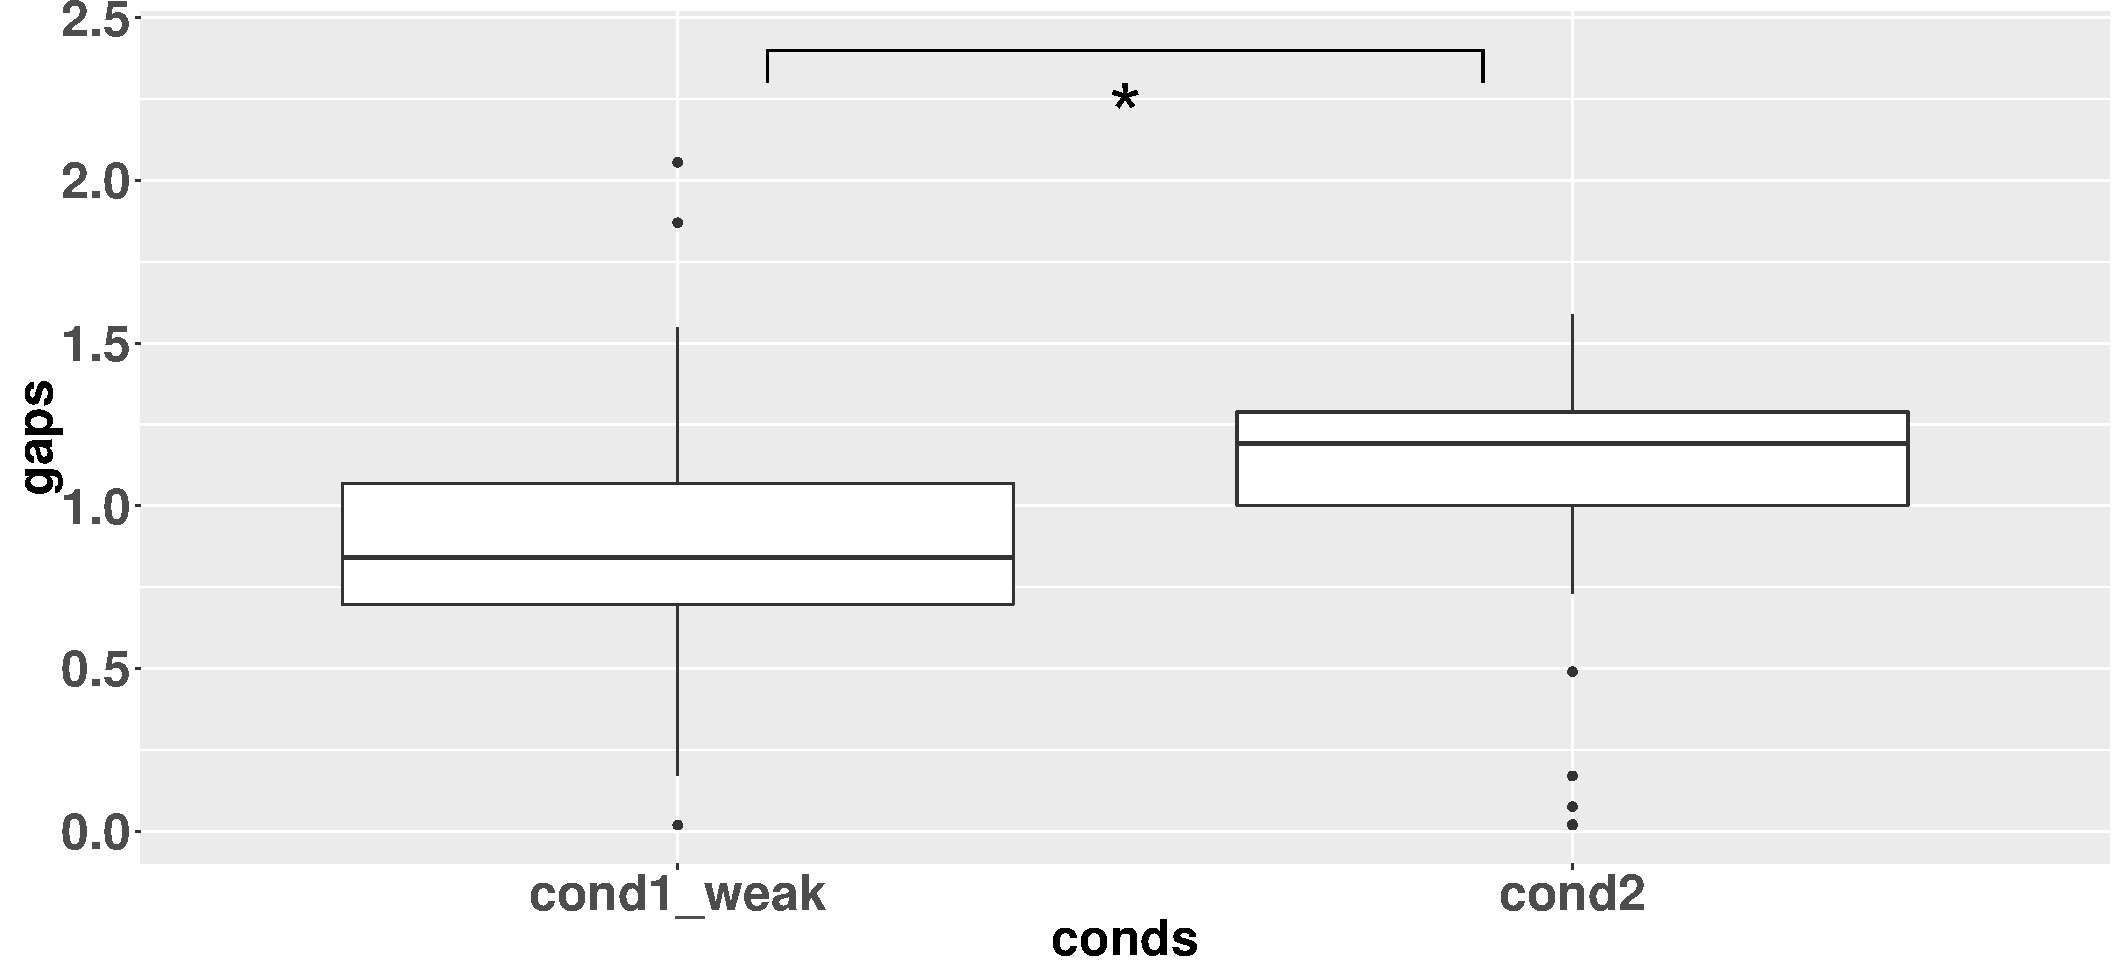
\includegraphics[width=\linewidth]{figure/boxTransitionsUA.pdf}
\caption{Durations of silence during User to Agent transitions (gaps in seconds).}
\label{box_ua}
\end{figure}

\begin{figure}
\centering
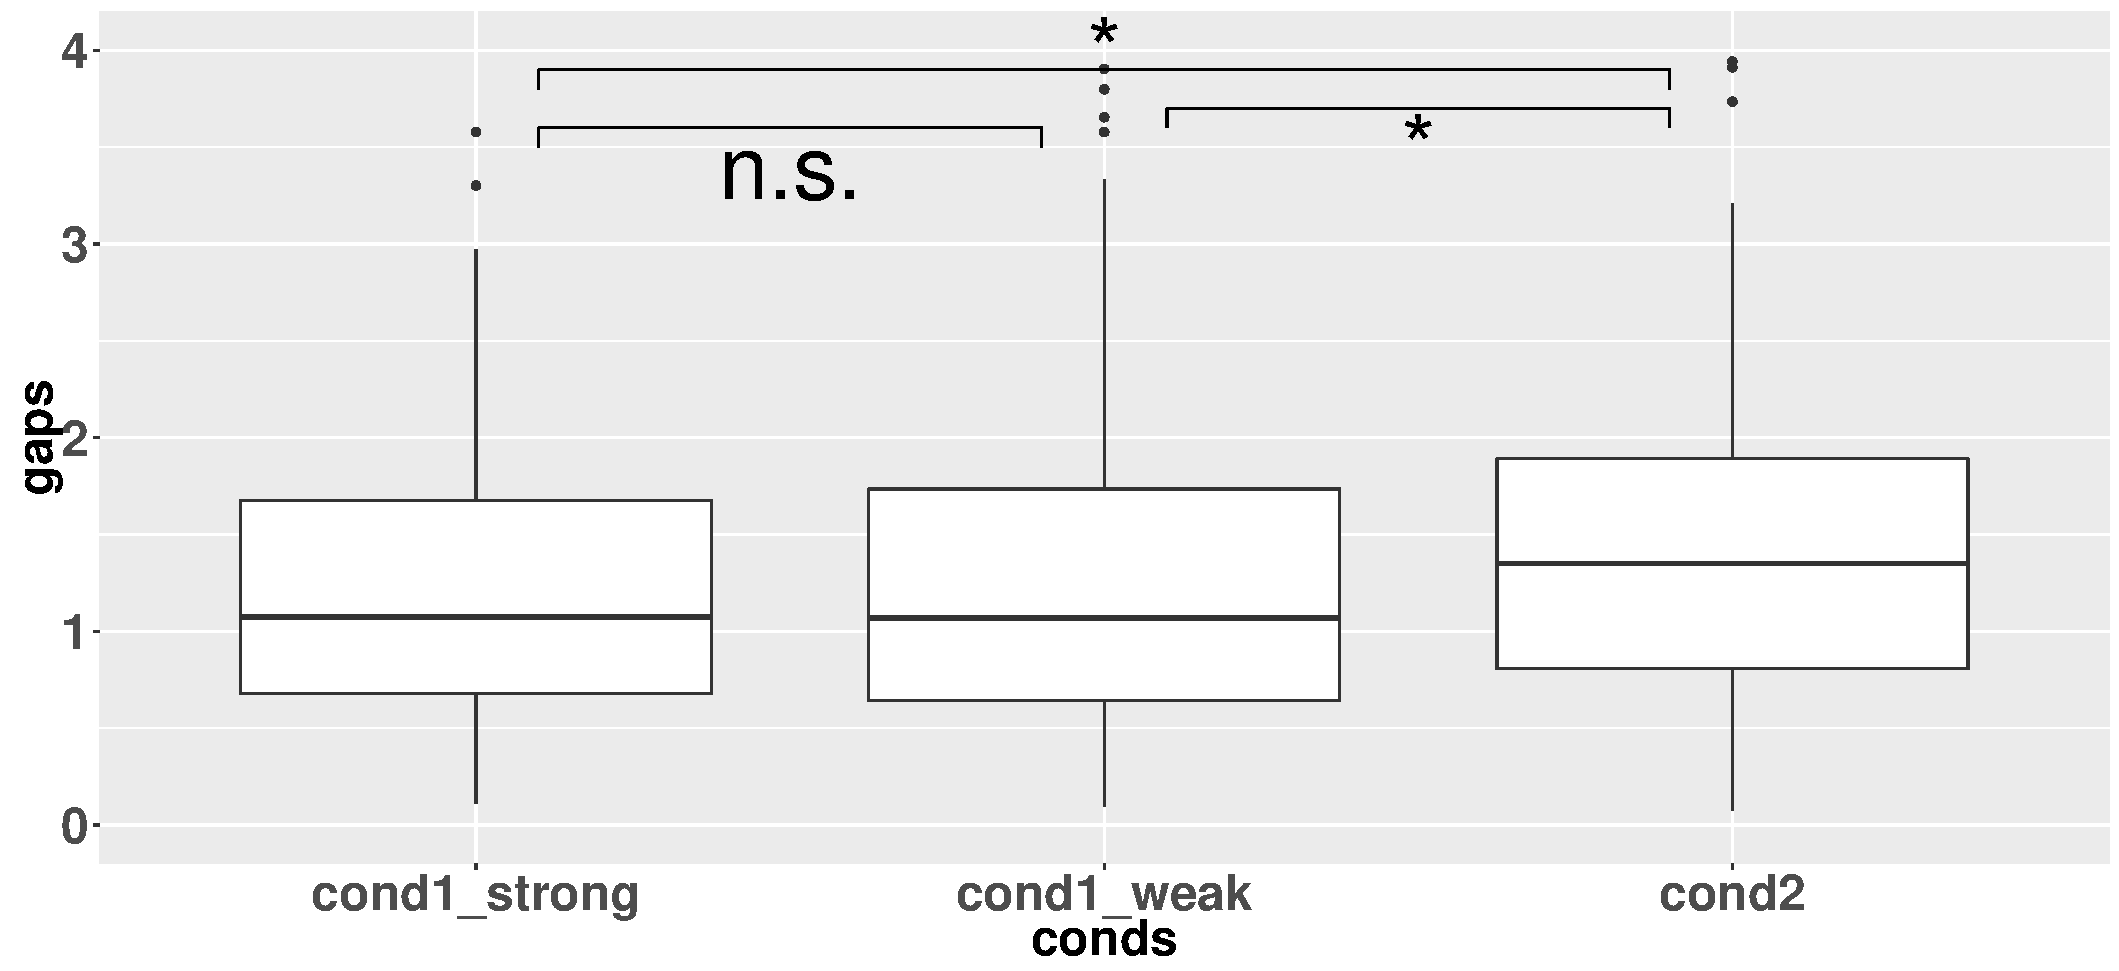
\includegraphics[width=\linewidth]{figure/boxTransitionsAU.pdf}
\caption{Durations of silence during Agent to User transitions (gaps in seconds).}
\label{box_au}
\end{figure}


We first analyzed the duration of the transitions, distinguishing user to agent transitions from agent to user ones (Figures \ref{box_ua} and \ref{box_au}).
 We observed first a high number of mistakes in the detection of user's end of turns, whatever the condition, with almost 50 \% of transitions having at least slight overlaps.  
%The repartition of the user to agent transitions is shown on figure \ref{box_ua}, and the repartition of agent to user transitions is shown on the figure \ref{box_au}. 

These results show that for the condition 1 the agent took the turn more rapidly (average: 840 ms) compared to the second condition (1.19 s), the difference being significant (p<0.05). The difference was also significant (p<0.05) for the agent-user transitions: in condition 1 the mean duration of silence was 1.11 s and 1.39 s for the second one. 
In addition, the pitch of the user was significantly greater than the mean pitch of the participant during conflictual moments, for condition 1 Strong.
 %to these transition duration values, the pitch variation of the participants was measured during interruptions by the agent. The results showed that the pitch of the user was significantly greater than the mean pitch of the participant during conflictual moments, for the condition 1 ``Strong".

% Comment peut-on expliquer que la durée moyenne de transition soit le double du seuil de détection de la fin de tour de l'utilisateur ?
% À faire : valeur moyenne de pitch supérieure aussi lors des overlaps de l'agent pour les autres conditions, différences de perception qui pourrait laisser penser une différence de traitement ?
% Comportement de l'agent : est-ce que l'utilisateur a beaucoup interrompu l'agent ?


\subsection{Discussion}

The results of our questionnaire do not seem to show effects of the turn-taking behavior on the user experience during interaction. The results of the questionnaire were compared to behavioral analysis showing that the user produced a significant but weak reaction when the agent interrupted him, but when varying the way the agent took turn (waiting the end of the user's turn or interrupting the user) between the conditions 1 ``weak" and 1 ``strong" we did not find modifications of the silence duration of agent to user transitions. 

At the end of the experiment, we collected the oral impressions of the participants on the interaction. Participants reported less categorical impressions towards the interruptions of the user than what has been observed in the responses of the questionnaires. Six participants explicitly mentionned that they perceived the interruptions of the agent as non-voluntary, on the oppsite, thirteen participants perceived at least some interruptions as voluntary. Among these thirteen participants, four participants judged these interruptions as coherent and credible given the dialog context, and five participants associated these interruptions to the fact that the agent did not agree or tried to impose its own ideas. Finally, among those thirteen participants, five participants judged those interruptions as humanlike. Nevertheless, these perception of the interruption did not conducted to more positive impressions about the interaction such a increasing naturality or credibility. One of the participants we interviewed after the experiment reported a rage feeling linked to the incessant interruptions of the agent, and two participants reported that they were annoyed by these interruptions. The results of the questionnaire have also shown that the subjects perceived the agent as strongly reactive and have scarcely noticed the presence of awkward silences during the conversation. When these moments of silence were perceived, they were considered as not natural, even if two participants perceived it as credible and linked to an agent that thought at what it wanted to say. This non natural character of awkward silences could be linked to the fact that the interaction was only audio preventing the agent to provide visual feedback to the user. 

The high rate of end of turn detections by the two models (50 \% of user-agent transitions) can partially explained by the voice activity detector used to detect the moments were the user spoke, showing an important number of moments were no voice was detected whereas the user actually spoke. The fact that the participants seemed not disturbed by the relatively high silence duration of user to agent transitions support the idea that the latter does not expect optimal turn transitions from the agent. The reports collected from the interviews of the participants tend to show that those interruptions can give an impression of smoothness and immersion in the dialogue, but, as the participants often mentionned the interruptions of the agent related to the dialog, to the condition that the interruption should be coherent to the dialog context and what the agent has to say. Finally, the lack of distinction between interruptions, those that were due to mistakes in the detection of the user end of turn and those that were voluntary could be due to difficulties of the participants to perceive the prosodic variations of the agent. These difficulties could come from the quality of the tts voice we used, participants having often reported the bad quality of the voice. 

